\documentclass[a4paper,12pt]{report}
% Importação de pacotes

\usepackage[T1]{fontenc}        % Pacote para usar tabela ASCII
\usepackage[utf8]{inputenc}     % Pacote para usar Unicode
\usepackage[portuguese]{babel}      % Seta o idioma para pt-BR

\usepackage{geometry}           % Controlar as margens da página
\geometry{top=30mm,bottom=20mm,left=30mm,right=20mm}  


%AJUSTE DO IDIOMA
\usepackage[utf8]{inputenc} %uso de ACENTOS
\usepackage[portuguese]{babel} % IDIOMA do documento
\usepackage[T1]{fontenc} % hifenização de pacotes acentuados

%PACOTES GERAIS
\usepackage{graphicx}               %habilita o uso de FIGURAS
\graphicspath{{./img/}}         %procura figuras na subpasta indicada
\usepackage[shortlabels]{enumitem}  %Permite mudar a forma de enumerar
\usepackage{multirow}       % Mesclar células na vertical
\usepackage{geometry}       % Controlar as margens da página
\usepackage{amsmath}        % macros de matemática, como dfrac{}{}
\usepackage{amssymb}        % símbolos matemáticos
\usepackage{wrapfig}        % Figuras junto de texto
\usepackage{tikz}           % Figuras tikz
\usepackage{comment}        % Ambiente de comentário
\usepackage{lastpage}       % Uso da macro LastPage para numerar a página
\usepackage{fancyhdr}       % Cabeçalho personalizado
\usepackage{fancybox}


%AJUSTE DAS FUNÇÕES TRIGONOMÉTRICAS
\providecommand{\sin}{} \renewcommand{\sin}{\mathrm{sen\,}}
\providecommand{\tan}{} \renewcommand{\tan}{\mathrm{tan\,}}
\providecommand{\cos}{} \renewcommand{\cos}{\mathrm{cos\,}}




\usepackage[sorting=nty, style=abnt,natbib=true, backend=biber]{biblatex}    % Importa o pacote bibTeX para a bibliografia
\addbibresource{bibliografia.bib}                                           % Importa o arquivo que contém a bibliografia

 % Hiperlinks no documento
\usepackage{hyperref}          
\hypersetup{
	colorlinks=true,
	linkcolor=black,
	filecolor=magenta,      
	urlcolor=black,
	citecolor=black,
}
\urlstyle{same}


\usepackage[dvipsnames]{xcolor} %uso de cores no texto, \color{cor} dentro de um bloco para colorir ele. 
%\definecolor{mypink2}{RGB}{219, 48, 122}
%pagecolor{cor}


\usepackage{enumitem}           % Permite personalizar o enumerate

\usepackage{setspace}           % Espaçamento entre linhas

% Macros de Título, Autor e Data
\title{Notas de Aula\\Matemática III}
\author{Fábio Dantas}
\date{\today}


% Ambiente de citação
\renewenvironment{quotation}
  {\small\list{}{\rightmargin=0.1cm \leftmargin=4cm \topsep=1.5\baselineskip}%
   \item\relax}
  {\endlist}

\def\signed #1{{\leavevmode\unskip\nobreak\newline
  \hbox{}\nobreak #1 %
  \hfil\parfillskip=0pt \finalhyphendemerits=0 \endgraf}}

\newsavebox\mybox
\newenvironment{citacao}[1]
  {\savebox\mybox{#1}\begin{quotation}}
  {\signed{\usebox\mybox}\end{quotation}}



\begin{document}

\onehalfspacing

\maketitle          % Produz a capa do documento

\tableofcontents    % Produz o sumário

% Faço o input de cada capítulo separado
\chapter{Grandezas e unidades de medidas}
% Grandezas e unidades de medidas: noções de instrumentos de medidas, unidades de medidas decimais e não decimais (medidas de comprimento, de superfícies, de capacidade, de tempo, dentre outros). Notação científica para expressar medidas.

\par Oi. Tentativa de inserir uma fórmula no texto $\displaystyle \lim_{x\rightarrow 10} x^2-2x+5$. Continuando o texto e uma fórmula em destaque. $$ax^2+bx+c=0 \Leftrightarrow x=\frac{-b \pm \sqrt{b^2-4ac}}{2a}.$$

\par Nova tentativa dessa vez comparando $\frac{2}{3}$ com $\dfrac{2}{3}$.

\section{Exercícios}
\begin{enumerate}[label=\textbf{\arabic*}.]
    \item Pergunta 1;
    \begin{enumerate}[label=\alph*)]
        \item item 1;
        \item item 2;
        \item item 3.
    \end{enumerate}
    \item Pergunta 2;
    \item Pergunta 3;
\end{enumerate}

\section{Citações}
Um texto qualquer que precede. Segundo \citet[p. 19]{manson2017sutil} "Melhor coisa do mundo é tocar o foda-se". Mais um texto para citação antes, pois segundo \citet[p. 10]{fabiodantas} ``Pior seria se pior fosse''. Ou ainda "A medida de amar é amar sem medida" \citep[p. 12]{fabiodantas}. Por fim, como dizia \citet[p. 8]{huff2016mentir} a melhor maneira de mentir é com estatística.

\begin{citacao}{\citep[p.50]{fabiodantas}}
    "Sed ut perspiciatis unde omnis iste natus error sit voluptatem accusantium doloremque laudantium, totam rem aperiam, eaque ipsa quae ab illo inventore veritatis et quasi architecto beatae vitae dicta sunt explicabo. Nemo enim ipsam voluptatem quia voluptas sit aspernatur aut odit aut fugit, sed quia consequuntur magni dolores eos qui ratione voluptatem sequi nesciunt. Neque porro quisquam est, qui dolorem ipsum quia dolor sit amet, consectetur, adipisci velit, sed quia non numquam eius modi tempora incidunt ut labore et dolore magnam aliquam quaerat voluptatem. Ut enim ad minima veniam, quis nostrum exercitationem ullam corporis suscipit laboriosam, nisi ut aliquid ex ea commodi consequatur? Quis autem vel eum iure reprehenderit qui in ea voluptate velit esse quam nihil molestiae consequatur, vel illum qui dolorem eum fugiat quo voluptas nulla pariatur?"
\end{citacao}

\begin{figure}[h!]
	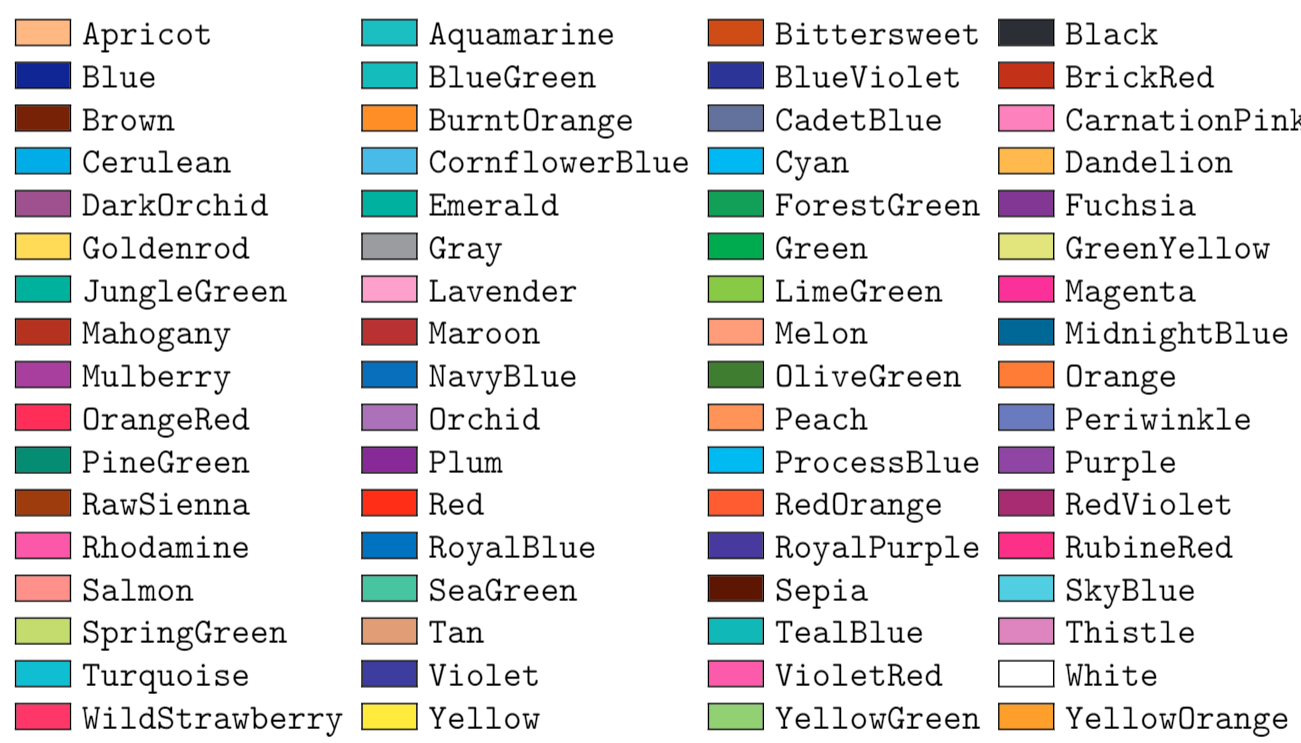
\includegraphics[width=\linewidth]{OLxcolorList2}
\end{figure}



%\input{txt/cap-razao}
%\chapter{Introdução à Teoria dos Conjuntos}
% Introdução à Teoria dos Conjuntos: conceituação e operações com conjuntos com ênfase na resolução de problemas.

Oi 3.

%\chapter{Conjuntos Numéricos}
%Conjuntos numéricos: estudo dos números naturais, inteiros, racionais, reais com ênfase em suas propriedades e operações. Módulo de um número real. Operações com intervalos reais.

Oi 4. 
%\chapter{Introdução ao conceito de Funções}
% Introdução ao conceito de funções: função como relação de dependência entre duas grandezas, definição de função como uma relação entre dois conjuntos, função definida por mais de uma sentença, representações gráficas, algébricas e por meio de tabelas. Função injetora, função sobrejetora e função bijetora. Função composta e função inversa.

Oi 5.
%\chapter{Função Afim}
%  Função afim: conceituação da função afim, taxa de variação, equações do 1º grau, zero da função, gráficos, estudo do sinal, inequações do 1º grau. Aplicações.

Oi 6. \cite{greenwade93}
%\chapter{Função Quadrática}
% Função quadrática: conceituação da função quadrática, equações do 2º grau, zeros da função, estudo do gráfico, máximos e mínimos, estudo do sinal e inequações. Aplicações.

Oi 7.
%\chapter{Função Exponencial}
% Função Exponencial: revisão de potenciação, de radiciação e propriedades. conceituação algébrica da função exponencial, estudo do gráfico, equações, inequações. Aplicações.

Oi 8.

%\chapter{Função Logarítmica}
% Função logarítmica: definição, consequência da definição, propriedades operatórias. conceituação algébrica da função logarítmica, estudo do gráfico, equações, inequações. Aplicações.

Oi 9.
%\chapter{Tópicos de Geometria Plana}
% Tópicos de Geometria Plana: teorema de Thales, semelhança de figuras planas, teorema de Pitágoras.

Oi 10. 
%\chapter{Introdução à Trigonometria}
% Introdução à Trigonometria: razões trigonométricas no triângulo retângulo, leis dos senos e dos cossenos com ênfase na conceituação e nas aplicações.

Oi 11.

% Bibliografia
%\singlespacing
\printbibliography[heading=bibintoc]

\end{document}
